\newpage 
\section{Embedding policy, practice and supports to advance academic and research careers}
\label{sec:academic}

This section explicitly considers research staff to be those who actively partake in the research itself. Those staff members that provide professional, administrative and managerial support to researchers are considered in the subsequent section.

\subsection{Reflecting on recruitment practices in the department}


\instr{

\begin{prompt}
\setlength\tabcolsep{6pt} 
\begin{tabu} to \textwidth {@{} X[9] X X }
     \multirow{2}{=}{Recruitment to academic and research posts in the department adheres to institutional policy on recruitment, which includes gender-balanced panels and training for assessors } 
     & \textbf{Yes} & \textbf{No}  \\
     &  \XBox & \Square  \\[.1in] 

\end{tabu}
\setlength\tabcolsep{0pt} 
\end{prompt}
If you answered `no', please comment.
}



\subsection{Provide three years of data on application, shortlist, and appointment rates for recruitment by gender and grade. Where data suggests opportunity for improvement, comment and reflect. Include any other relevant information relating to recruitment processes and practice for academic and research posts in the department. }


\subsubsection{Academic posts}
Table~\ref{tab:equality:recruitment:academic} presents recruitment data for the years 2017/18 and 2018/19; no recruitment took place during the year 2019/2020. 
%Recruitment into academic posts took place during the years 2017/18 and 2018/19, there was no recruitment during the year 2019/20. 
There were nine academic appointments during these three years.
%(see Table~\ref{tab:equality:recruitment:academic}). 
The recruitment process into academic posts is centrally managed by \ac{HR}. % and differs between professorial posts and non-professorial posts. 
% In general, the 
%The School provides text for advertisements, nominates members of the selection committee to the Head of College, who nominates the Chair of the selection committee, and nominates external assessors, typically academics from other universities in Ireland or abroad, with relevant discipline-specific expertise. A HR representative is in attendance during shortlisting and interview.

The data show that the school received significantly fewer applications from female applicants compared to male applicants, in particular for the senior position of Professor. 
Although there were female applicants in year 2017/18, no women were appointed to any of the four available posts. 
The next year was more positive towards gender balance, where 3 out of 5 positions were filled with female applicants. 

\begin{tabbox}{!th}
\caption{Gender equality and selection committees for academic positions}
\label{tab:selection:acad}
\footnotesize 
\sisetup{
    group-digits=all,
    group-minimum-digits=4,
    group-separator = {,},
    table-format=4.1,
    mode=text,
    reset-text-series = false, 
    text-series-to-math = true,
    reset-text-family = false, 
    text-family-to-math = true
}
\begin{tabular}{p{2cm}
                p{9.4cm}
                R{0.7cm}
                R{0.7cm}
                !{\qquad}
                S[table-format=2.0\%]
                }
\toprule
    {Year} & 
    {Competition} & 
    \multicolumn{3}{c}{{\makecell{Selection Committee}}} \\
    \cmidrule{3-5}
    & & {F} & {M} & {\%F}\\
\midrule

2017/18 & Professor of Computer Science & 3 & 5 & 38\% \\ 
\cdashline{2-5}
& Lecturer in Computer Science & 3 & 3 & 50\% \\
\cdashline{2-5}
& Lecturer in Computer Science & 3 & 3 & 50\% \\
\hdashline
2018/19 & Lecturer in Computer Science (x2) & 2 & 4 & 33\% \\
\cdashline{2-5}
& Lecturer in Computer Science (BA Psychology) & 3 & 2 & 60\%\\
\cdashline{2-5}
& Lecturer in Computer Science (BA Digital Humanities) & 3 & 2 & 60\% \\
\cdashline{2-5}
& Lecturer in Computer Science & 2 & 3 & 40\% \\
\midrule
Total & & 19 & 22 & 46\% \\
\bottomrule

\end{tabular}
{
\\[2mm]
\sffamily Note: No recruitment in 2019/2020.
}
\end{tabbox}




\begin{tabbox}{!th}
\caption{Gender equality and academic recruitment}
\label{tab:equality:recruitment:academic}
\footnotesize 

\begin{tabular}{P{1.5cm}P{4.6cm}C{1.0cm}
                                C{0.9cm}
                                R{0.7cm}
                                p{0.2cm}
                                C{1.0cm}
                                C{0.9cm}
                                R{0.7cm}
                                p{0.2cm}
                                C{1.0cm}
                                C{0.9cm}
                                R{0.7cm}}
\toprule
    {Year} & 
    {Competition} & 
    \multicolumn{3}{c}{{\makecell{Applicants}}} && 
    \multicolumn{3}{c}{{\makecell{Shortlisted}}} &&
    \multicolumn{3}{c}{{\makecell{Appointed}}}\\
    \cmidrule(l){3-5}\cmidrule(l){7-9}\cmidrule(l){11-13} 
    & & {F} & {M} & {\%F} && {F} & {M} & {\%F} && {F} & {M} & {\%F}\\
\midrule

2017/18 & Professor of Computer Science & 2 & 25 & 7\% && 0 & 7 & 0\% && 0 & 2 & 0\%\\ 
\cdashline{2-13}
& Lecturer in Computer Science & 7 & 15 & 32\% && 4 & 3 & 57\% && 0 & 1 & 0\%\\
\cdashline{2-13}
& Lecturer in Computer Science & 4 & 24 & 14\% && 0 & 7 & 0\% && 0 & 1 & 0\%\\
\hdashline
2018/19 & Lecturer in Computer Science (x2) & 9 & 44 & 17\% && 2 & 7 & 22\% && 1 & 1 & 50\%\\
\cdashline{2-13}
& Lecturer in Computer Science (BA Psychology) & 7 & 12 & 37\% && 3 & 3 & 50\% && 1 & 0 & 100\%\\
\cdashline{2-13}
& Lecturer in Computer Science (BA Digital Humanities) & 8 & 17 & 32\% && 2 & 4 & 33\% && 1 & 0 & 100\%\\
\cdashline{2-13}
& Lecturer in Computer Science & 0 & 6 & 0\% && 0 & 1 & 0\% && 0 & 1 & 0\%\\
\midrule 
Total & & 37 & 143 & 21\% & & 11 & 32 & 26\% && 3 & 6 & 33\% \\
\bottomrule
\end{tabular}
{
\\[2mm]
\sffamily Note: No recruitment in 2019/2020.
}
\end{tabbox}




%While there was a high percentage of female academic staff appointments during 2018/19, one of those staff has since left the school. 
At the time of writing, the School has no female academic staff in senior roles, i.e. \ac{SL} and above (see Table~ \ref{tab:acresstaff}). 
%The percentage of female academic staff in the School is the lowest of all Computer Science departments in Irish universities. 
%The low number of female academic staff has also impacted the staff survey data, as only one female academic staff member responded to the survey, making it impossible to present statistics based on the survey. Therefore, most of the consultation information in the following is presented in a qualitative manner.
%
%During the academic year 2020/21, the school advertised for the position of Professor (scale 2) in Human Centred Computing, providing an opportunity to address the issue of low numbers of academic staff to some extent. The recruitment process yielded two appointable applicants, both female, but both declined the offer in the end. 
The School is committed to addressing the staff gender imbalance and avails of every opportunity to do so. For example, it has applied to the \ac{SALI} chair initiative in 2019 and 2020 to fund a female professorship for the School. However, the School's proposals were not successful. 
%The School will continue to monitor such initiatives as they arise and will apply for every opportunity.

%One way to increase the number of female academic staff is through an increase the number of female applicants for open positions. 
During the academic staff focus group discussion, colleagues noted that the language of recruitment advertisements impacts on whether women are attracted to the position or not:

\begin{myquote}
``... can write a job advert in a way that discourages women from applying – it's the language you use ...''
\end{myquote}

The School will, going forward, carefully draft with the help of the EDI unit, advertisements for academic positions that may appeal better to women and will also encourage female research staff to apply (Action~\ref{action:acad:marketing}). Furthermore, the School will make an effort to search internationally to target suitable female candidates and encourage them to apply (Action~\ref{action:acad:femaleonly}).

\newcommand{\actacadmarketing}{%Action 2.1 
Improve the advertising text for staff positions to make it more appealing to under represented genders.}
\begin{actionblock}{\ksspace{}Improve Advertising Text}{acad:marketing}
\actacadmarketing
\hfill{
    \hypersetup{hidelinks}
    \hyperlink{c2}{\gotoactionsymbol{}}
}
\end{actionblock}


\newcommand{\actacadfemaleonly}{%Action 2.2
Actively target suitable female academics to apply.}
\begin{actionblock}{\ksspace{}Target Suitable Female Academics}{acad:femaleonly}
\actacadfemaleonly
\hfill{
    \hypersetup{hidelinks}
    \hyperlink{c1}{\gotoactionsymbol{}}
}
\end{actionblock}

\subsubsection{Research posts}
Table~\ref{tab:equality:recruitment:research} shows aggregate data on research staff recruitment during the three relevant academic years 2017/18 – 2019/20, organised by position/grade.
On average there are 20\% female applicants for research positions with similar percentages being shortlisted and appointed. 
%While the proportion of applicants is similar to the proportion of females appointed, globally, of women in Computer Science, the performance of the school appears to be only preserving the status quo on gender diversity in academia rather than improving it. 

\begin{tabbox}{!th}

      
\footnotesize 
\caption[Gender equality and research staff recruitment, aggregated by position/grade]{Gender equality and research staff recruitment, aggregated by position/grade. * marks incomplete data.}
\label{tab:equality:recruitment:research}
\sisetup{
    group-digits=all,
    group-minimum-digits=4,
    group-separator = {,},
    mode=text,
    reset-text-series = false, 
    text-series-to-math = true,
    reset-text-family = false, 
    text-family-to-math = true
}

\begin{tabular}{P{1.5cm}
                P{3.8cm}
                !\quad
                S[table-format=2.0]
                !\quad
                S[table-format=3.1]
                !\quad
                S[table-format=2.1\%]
                p{0.5cm}
                S[table-format=2.0]
                !\quad
                S[table-format=3.1]
                !\quad
                S[table-format=2.1\%]
                p{0.5cm}
                S[table-format=2.0]
                !\quad
                S[table-format=3.1]
                !\quad
                S[table-format=2.1\%]}
\toprule
    Year & 
    Role (number of positions) & 
    \multicolumn{3}{c}{\makecell{Applicants}} & &
    \multicolumn{3}{c}{\makecell{Shortlisted}} & &
    \multicolumn{3}{c}{\makecell{Appointed}}\\
    \cmidrule{3-5}\cmidrule{7-9}\cmidrule{11-13} 
    & & {F} & {M} & {\%F} && {F} & {M} & {\%F} && {F} & {M} & {\%F}\\
\midrule

%2017/18 & Senior post-doctoral researcher & 0 & 1 & 0\% & 0 & 1 & 0\% & 0 & 1 & 0\%\\
2017/18 & Post-doctoral researcher (2) & 1 & 1 & 50.0\% && 1 & 1 & 50.0\% && 1 & 1 & 50.0\%\\
\cdashline{2-13}
& Senior post-doctoral researcher (3) & 0 & 3 & 0.0\% && 0 & 3 & 0.0\% && 0 & 3 & 0.0\%\\
\cdashline{2-13}
%& Systems and high performance computing lead at Insight (senior research coordinator) 
& Senior research coordinator (1)
& 0 & 1 & 0.0\% && 0 & 1 & 0.0\% && 0 & 1 & 0.0\%\\
\hdashline
2018/19 & Post-doctoral researcher (9) & 1 & 8 & 11.1\% && 1 & 8 & 11.1\% && 1 & 8 & 11.1\% \\
\cdashline{2-13}
& Senior post-doctoral researcher (4) & 1 & 3 & 25.0\% && 1 & 3 & 25.0\% && 1 & 3 & 25.0\%\\
\cdashline{2-13}
& Research fellow (1) & 0 & 1 & 0.0\% && 0 & 1 & 0.0\% && 0 & 1 & 0.0\%\\
\cdashline{2-13}
& Research assistant (1) & 0 & 1 & 0.0\% && 0 & 1 & 0.0\% && 0 & 1 & 0.0\%\\
\cdashline{2-13}
& Senior Research Coordinator (3) & 0 & 3 & 0.0\% && 0 & 3 & 0.0\%  && 0 & 3 & 0.0\%\\
\cdashline{2-13}
& Research Support officer (1) & 1 & 0 & 100.0\% && 1 & 0 & 100.0\%  && 1 & 0 & 100.0\%\\
\hdashline
2019/20 & Post-doctoral researcher (9) & 23 & 137 & 0.0\% && * & * & * && 0 & 8 & 0.0\% \\
\cdashline{2-13}
& Senior post-doctoral researcher (4) & 4 & 19 & 82.6\% && * & * & * && 1 & 1 & 50.0\%  \\
\cdashline{2-13}
& Post-doctoral / Senior postdoctoral researcher (3)  & 7 & 62 & 10.1\% && * & * & * && 0 & 2 & 0.0\%   \\
\cdashline{2-13}
& Research coordinator (2) & 9 & 1 & 10.0\% && * & * & * && 0 & 0 & 0.0\% \\
\cdashline{2-13}
& Senior research coordinator (1) & 2 & 3 & 60.0\% && * & * & * && 0 &  1 & 0.0\% \\
\cdashline{2-13}
& Research assistant (1) & 2 & 3 & 60.0\% && * & * & * && 1 & 0 & 100.0\% \\
\cdashline{2-13}
& Research Support officer (1) & 3 & 10 & 76.9\% && * & * & * && 1 & 0 &  100.0\%\\

\midrule
& Total (46) & 48 & 193 & 20.0\% && * & * & * && 8 & 30 & 21.0\%\\

\bottomrule
\end{tabular}


\end{tabbox}



The staff survey revealed that job descriptions for research positions were not always well-defined. Similar to the academic post advertisements (Action~\ref{action:acad:marketing}), we will carefully review job descriptions and `gender-proof' the advertising text for research positions.
We will also advertise through a more diverse set of channels to make sure more female candidates are reached, increasing the number of female applicants, e.g. Women in AI, IEEE Women in Engineering network, etc.

%We need to improve the pool of suitable female researchers that find academic posts attractive. 
In addition to the actions listed in Section~2.\ref{sec:overview} 
we will identify female PhD students and research staff with an interest in an academic research career to help them develop their careers to make them strong candidates for future academic positions (Action~\ref{action:acad:personalplan}).

% check if sentence below could go into Kieran's section
% We are already addressing gender diversity at PhD level through our two SFI Centres for Research Training, which have targets for at least 40\% female PhD students. 






%\newcommand{\actacadfemalestudents}{%Action 2.4 - merge with action in section 1
%Create a specific initiatives to help attract more female undergraduate and graduate students}
%\begin{action}[label=action:acad:femalestudents]{}
%\actacadfemalestudents
%\hfill{
%    \hypersetup{hidelinks}
%    \hyperlink{c3}{\gotoactionsymbol{}}
%}
%\end{action}

\newcommand{\actacadpersonalplan}{%Action 2.3 
Support researchers, in particular female, with personal development plan and career support}
\begin{actionblock}{\ksspace{}Support Staff with Personal Development Plan}{acad:personalplan}
\actacadpersonalplan
\hfill{
    \hypersetup{hidelinks}
    \hyperlink{c4}{\gotoactionsymbol{}}
}
\end{actionblock}

While the University has clear guidelines for the recruitment process of academic positions in terms of gender-balance of the selection committee, %the recruitment process for academic posts is specified in UCC regulations based on the Universities Act 1997, 
%there are less clear guidelines for recruitment into postdoctoral or research fellow (apart from senior research fellow) posts. While gender-balanced committees are a requirement for academic positions, 
no such guidelines are available for committees recruiting for research positions. 

%%*** FIG 1 HERE ***
\begin{tabbox}[5cm]{!th}
\caption{Selection committee gender balance research}
\label{tab:committee:gender:balance:research}
\footnotesize 

\sisetup{
    group-digits=all,
    group-minimum-digits=4,
    table-format=2.1,
    mode=text,
    reset-text-series = false, 
    text-series-to-math = true,
    reset-text-family=false, 
    text-family-to-math=true
}
\begin{tabular}{p{4cm}
                S[table-format=2.0\%]
                }
\toprule 
Gender & {\%}\\ 
\midrule 
Male & 78\%\\
\hdashline 
Female & 19\% \\
\hdashline 
Unknown & 3\% \\
\bottomrule 
\end{tabular}
\end{tabbox}

% \begin{SCtable}
% \caption{Committee gender balance research}
% \label{tab:committee:gender:balance:research}
% \footnotesize 
% \sisetup{
%     group-digits=all,
%     group-minimum-digits=4,
%     table-format=2.1,
%     mode=text,
%     reset-text-series = false, 
%     text-series-to-math = true,
%     reset-text-family=false, 
%     text-family-to-math=true
% }
% \begin{tabular}{p{4cm}
%                 S[table-format=2.0\%]
%                 }
% \toprule 
% Gender & {\%}\\ 
% \midrule 
% Male & 78\%\\
% \hdashline 
% Female & 19\% \\
% \hdashline 
% Unknown & 3\% \\
% \bottomrule 
% \end{tabular}
% \end{SCtable}

Table~\ref{tab:committee:gender:balance:research} shows that 19\% of recruitment committee members for research positions are female. However, both the available data and the staff survey indicated that many recruitment committees for research staff are often entirely male. 
%The primary reason is that almost all PIs in the School who are have much influence on who is hired, are male. 
While recruitment training is required for academic staff recruitment committees, there are no specific guidelines for research positions. Going forward, the School will require all academic and research staff engaged in recruitment for research positions to have had training for participation in selection committees (Action~\ref{action:acad:recruittraining}).


\newcommand{\actacadrecruittraining}{% not all staff involved in research recruitment have had recruitment training
Recruitment training for all staff engaged in recruitment for research positions.
}
\begin{actionblock}{\ksspace{}Recruitment Training for Research Positions}{acad:recruittraining}
\actacadrecruittraining
\hfill{
    \hypersetup{hidelinks}
    \hyperlink{c7}{\gotoactionsymbol{}}
}
\end{actionblock}

In order to enhance the gender representation of selection committees for research positions in the School, we will create guidelines for gender representation in recruitment of research staff in line with the university-wide requirements for academic staff (Action~\ref{action:acad:balancecommittees}). %, \todo{but without overburdening female staff members.}

\newcommand{\actacadbalancecommittees}{
Endaveour gender balanced and diverse selection committees for research positions.
}
\begin{actionblock}{\ksspace{}Gender Balanced Selection Committees}{acad:balancecommittees}
\actacadbalancecommittees
\hfill{
    \hypersetup{hidelinks}
    \hyperlink{c5}{\gotoactionsymbol{}}
}
\end{actionblock}



During the academic staff focus group, concern was also expressed that recruitment policies do not provide means for accounting for gaps in candidates CVs related to maternity leave, caring responsibilities, etc. 

\begin{myquote}
``There isn’t a guideline, ... that says, look if you have had a family break of any kind, male or female … you have this opportunity to describe it … so that if you have gaps in your CV, you can explain them, because gaps in a CV are a red flag if they're not explained.''
\end{myquote}

%In fact, some of these aspects cannot be explored during interviews as they are not permissible questions. 
As gaps in CV due to, for example, maternity or caring leave, tend to affect women more than men, we will carefully examine how we can within the University's interview guidelines, enhance the way we assess applicants for shortlisting and appointment (Action~\ref{action:acad:cvgaps}) to be inclusive of relevant career gaps.

\newcommand{\actacadcvgaps}{% note the label has changed to reflect the different action 
We will create an opportunity for all job applicants to provide \todo{Covid-19} and family related leave statements in their applications that they would like selection committees take into account.
}
\begin{actionblock}{\ksspace{}Consider Leave Statements}{acad:cvgaps}
\actacadcvgaps 
\hfill{
    \hypersetup{hidelinks}
    \hyperlink{c6}{\gotoactionsymbol{}}
}
\end{actionblock}




\subsection{Reflecting on academic promotion in your institution, answer the following: }

\instr{
\begin{prompt}
\setlength\tabcolsep{6pt} 
\begin{tabu} to \textwidth {@{} X[8] X X X }
     \multirow{2}{=}{Academic promotion processes, including eligibility criteria, are managed centrally by the institution} & \textbf{Yes} & \textbf{No}  & \textbf{N/A}\\
     &  \XBox & \Square  & \Square \\ 
\end{tabu}
\setlength\tabcolsep{0pt} 
\end{prompt}
}

\instr{If you answered ‘no’, please comment on the department’s role in academic promotions processes. If you answered ‘not applicable’, as prescribed promotion pathways are not in place in your institution, provide comment and reflection on alternative routes for academic career progression.}

\subsection{Provide three years of data on application and success rates for promotion by gender and grade and present results from staff consultation by gender. Where data suggests opportunity for improvement, comment and reflect}

% Academic promotion applications are invited from time-to-time university-wide, however, not many of these invitations have appeared in recent years. 
% Until recently, there was a defined but irregular process for academic promotions from Lecturer below the merit bar to Lecturer above the bar, and from Lecturer (above the bar) to \ac{SL}, and \ac{SL} to Professor (Scale 2). 
% There is no promotion process from Professor (Scale 2) to Full Professor/Chair (Professor Scale 1) in UCC. 
% The process used to be one through a university-wide competition, i.e., fulfilling all requirements did not imply actual promotion.
% The university has announced a new merit-based promotion scheme, but details have not been published at the time of writing.

%During the three years of data considered, only 
Only one call for promotions invitation was sent out during the three years under consideration (in 2018/19). Two male academic staff members applied for promotion to \ac{SL}, but were unsuccessful. % (see Table \todo{3}). 
No female academic staff were eligible for promotion during these three years. 
%Surprisingly, no academic staff of the school attended any of the briefing sessions on promotion during the three years from 2018 – 2021. 
There is no promotion process for research staff in UCC as all research positions are fixed-term. 

%*** TABLE 3 HERE ***

% Need to have some data from staff survey as well - current data incorrect though
The staff survey provided a clear message that staff are not happy with the lack of promotion opportunities. It also indicated that many of the respondents feel the promotion criteria and the process are not transparent and fair. Focus group participants expressed a similar sentiment of dissatisfaction. %also expressed strong dissatisfaction with promotion opportunities.

% quotes are not useful for this part of the presentation. I will see if I can extract better data from the staff survey
%\begin{myquote}
%``There is no promotion scheme... It seems to be an impossible process to ... become a professor in UCC. I’ve kind of given up hope, to be honest.''
%\end{myquote}

%\begin{myquote}
%``In essence, there is no realistic prospect of promotion whatsoever... ''
%\end{myquote}

%Focus group participants also felt that the recently introduced UCC Futures recruitment strategy, which prioritises recruitment in ten thematic research areas, further reduces their prospects of progressing to a more senior role, because their research areas do not align with the areas in the strategy. One focus group participant commented as follows:

%\begin{myquote}
%``I don’t think I’ll ever get a [more senior] position, ... I’m never going to get one of those because they do not align with my area of expertise.''
%\end{myquote}

%The lack of promotion opportunities is leading to a feeling of being ``hugely undervalued'' among staff relative to their academic peers in other countries, who at the same career stage have achieved associate/professor grades with less research impact. Participants described other negative impacts on morale across the university due to the lack of promotion opportunities:

%\begin{myquote}
%``I know people in other schools who essentially said, look, I’m going to give it another three or four years. I’ll continue my research. I’ll continue to apply for grants ... if I don't get promoted then that’s it for me. ...''
%\end{myquote}

%Participants also described the lack of promotion opportunities as a deterrent to women considering an academic career in Computer Science:

%\begin{myquote}
%``there's so many hoops that you have to jump through, like you have to do so many things to get promoted. ... if you want to attract people you need to have better working circumstances.''
%\end{myquote}

%Reflecting on the unsuccessful promotions and the fact that the female academic staff members have only been very recently, since 2017,  recruited and as such are only now eligible for promotion, 
At the time of writing, the University has announced a new promotion scheme for 2023. We will 
%Going forward, we will raise awareness of promotion opportunities and 
create a mentoring and support scheme where senior colleagues support academic staff in their preparation for promotion (Action~\ref{action:acad:mentoring}). 
%While the action is not gender specific, the promotion route is a good vehicle for addressing the gender imbalance at senior level.

\newcommand{\actacadmentoring}{
Create a mentoring and support scheme for academic staff who seek promotion.}
\begin{actionblock}{\ksspace{}Academic Mentoring Scheme}{acad:mentoring}
\actacadmentoring
\hfill{
    \hypersetup{hidelinks}
    \hyperlink{c10}{\gotoactionsymbol{}}
}
\end{actionblock}

%%%%%%  KS XXX this is duplicate action from above, commenting it out here.
%%%%%%
% % maybe move this action to another section, perhaps on what the school can do to support people.
% \newcommand{\actresmentoring}{%Action 2.6 
% Create a mentoring scheme for researcher to help them develop their careers}
% \begin{action}[label=action:acad:mentoring]{}
% \actacadmentoring
% \hfill{
%     \hypersetup{hidelinks}
%     \hyperlink{c10}{\gotoactionsymbol{}}
% }
% \end{action}


%

\begin{tabbox}{!th}
\caption{Gender equality and academic recruitment}
\label{tab:equality:recruitment:academic}
\footnotesize 

\begin{tabular}{P{1.5cm}P{4.6cm}C{1.0cm}
                                C{0.9cm}
                                R{0.7cm}
                                p{0.2cm}
                                C{1.0cm}
                                C{0.9cm}
                                R{0.7cm}
                                p{0.2cm}
                                C{1.0cm}
                                C{0.9cm}
                                R{0.7cm}}
\toprule
    {Year} & 
    {Competition} & 
    \multicolumn{3}{c}{{\makecell{Applicants}}} && 
    \multicolumn{3}{c}{{\makecell{Shortlisted}}} &&
    \multicolumn{3}{c}{{\makecell{Appointed}}}\\
    \cmidrule(l){3-5}\cmidrule(l){7-9}\cmidrule(l){11-13} 
    & & {F} & {M} & {\%F} && {F} & {M} & {\%F} && {F} & {M} & {\%F}\\
\midrule

2017/18 & Professor of Computer Science & 2 & 25 & 7\% && 0 & 7 & 0\% && 0 & 2 & 0\%\\ 
\cdashline{2-13}
& Lecturer in Computer Science & 7 & 15 & 32\% && 4 & 3 & 57\% && 0 & 1 & 0\%\\
\cdashline{2-13}
& Lecturer in Computer Science & 4 & 24 & 14\% && 0 & 7 & 0\% && 0 & 1 & 0\%\\
\hdashline
2018/19 & Lecturer in Computer Science (x2) & 9 & 44 & 17\% && 2 & 7 & 22\% && 1 & 1 & 50\%\\
\cdashline{2-13}
& Lecturer in Computer Science (BA Psychology) & 7 & 12 & 37\% && 3 & 3 & 50\% && 1 & 0 & 100\%\\
\cdashline{2-13}
& Lecturer in Computer Science (BA Digital Humanities) & 8 & 17 & 32\% && 2 & 4 & 33\% && 1 & 0 & 100\%\\
\cdashline{2-13}
& Lecturer in Computer Science & 0 & 6 & 0\% && 0 & 1 & 0\% && 0 & 1 & 0\%\\
\midrule 
Total & & 37 & 143 & 21\% & & 11 & 32 & 26\% && 3 & 6 & 33\% \\
\bottomrule
\end{tabular}
{
\\[2mm]
\sffamily Note: No recruitment in 2019/2020.
}
\end{tabbox}







\subsection{Reflecting on opportunities for staff development reviews, answer the following:}\label{sec:2e}

\instr{
\begin{prompt}
\setlength\tabcolsep{6pt} 
\begin{tabu} to \textwidth {@{} X[8] X X @{}}
     \multirow{2}{=}{The institution operates a development review process, or equivalent, for academic and research staff} & \textbf{Yes} & \textbf{No}  \\
     &  \XBox & \Square   \\ 
\end{tabu}
\setlength\tabcolsep{0pt} 
\end{prompt}
}

\instr{
If you answered ‘yes’, comment and reflect on the implementation of this institution-level process in the department. This should include: 
\begin{itemize}
\item	data on uptake by gender;
\item	results from staff consultation presented by gender;
\item	information on any additional department-level opportunities for staff to discuss professional development. 
\end{itemize}

\noindent If you answered ‘no’, provide detail on department-level opportunities for staff to discuss professional development, including data on uptake by gender and results from staff consultation presented by gender. 
}



\subsubsection{Uptake of staff development reviews}

UCC operates a \ac{PDRS}. The PDRS process is meant to apply to all staff, except for those staff with less than 50\% FTE, less than a year left on a contract, staff on probation, on long term sick leave, or within two years of retirement. During the process, which involves the \ac{HOS} for all academic staff and the line manager for research staff, development needs can be discussed. During the years 2017/18-20, there had been no formal PDR process. While the PDR process was due to restart in the academic year 2019/2020, these were further postponed due to the onset of the Covid-19 pandemic in March 2020. A new \ac{HOS} was appointed in September 2021 and the review process is now rescheduled for the new academic year 2022/23 (Action~\ref{action:acad:pdrs}).


\newcommand{\actacadpdrs}{%Action 2.18 
Restart PDRS process in school to review and assess staff development.}
\begin{actionblock}{\ksspace{}Restart PDRS Process}{acad:pdrs}
\actacadpdrs
\hfill{
    \hypersetup{hidelinks}
    \hyperlink{c13}{\gotoactionsymbol{}}
}
\end{actionblock}


\subsubsection{Training and Development Opportunities for Academic Staff}
UCC provides a broad spectrum of training and development programmes for academic and research staff. These include personal and professional development, management and leadership development, and staff wellbeing, which are coordinated by HR, the \ac{OVPRI}, and the Office of the VP for Teaching and Learning. 
%training on research and innovation processes, grant writing and management, etc. offered by the research office, as well as courses on teaching and learning provided by the office of the VP for Teaching and Learning. 
Table~\ref{tab:training:academic} 
shows the uptake of development opportunities by academic staff during the three years of data reporting. The low uptake of training by female academic staff is in part due to the fact that the School only has two female academic members. 
%While the uptake of these courses appears much higher for male academic staff compared to female staff, the data do not identify individuals, and therefore it is unclear how many individuals are captured by the data.

%%** TABLE 4 % table needs to be inserted
% \begin{table}[!ht]
%     \caption{Training uptake by academic staff by gender}
%     \label{tab:training:academic}
%     %%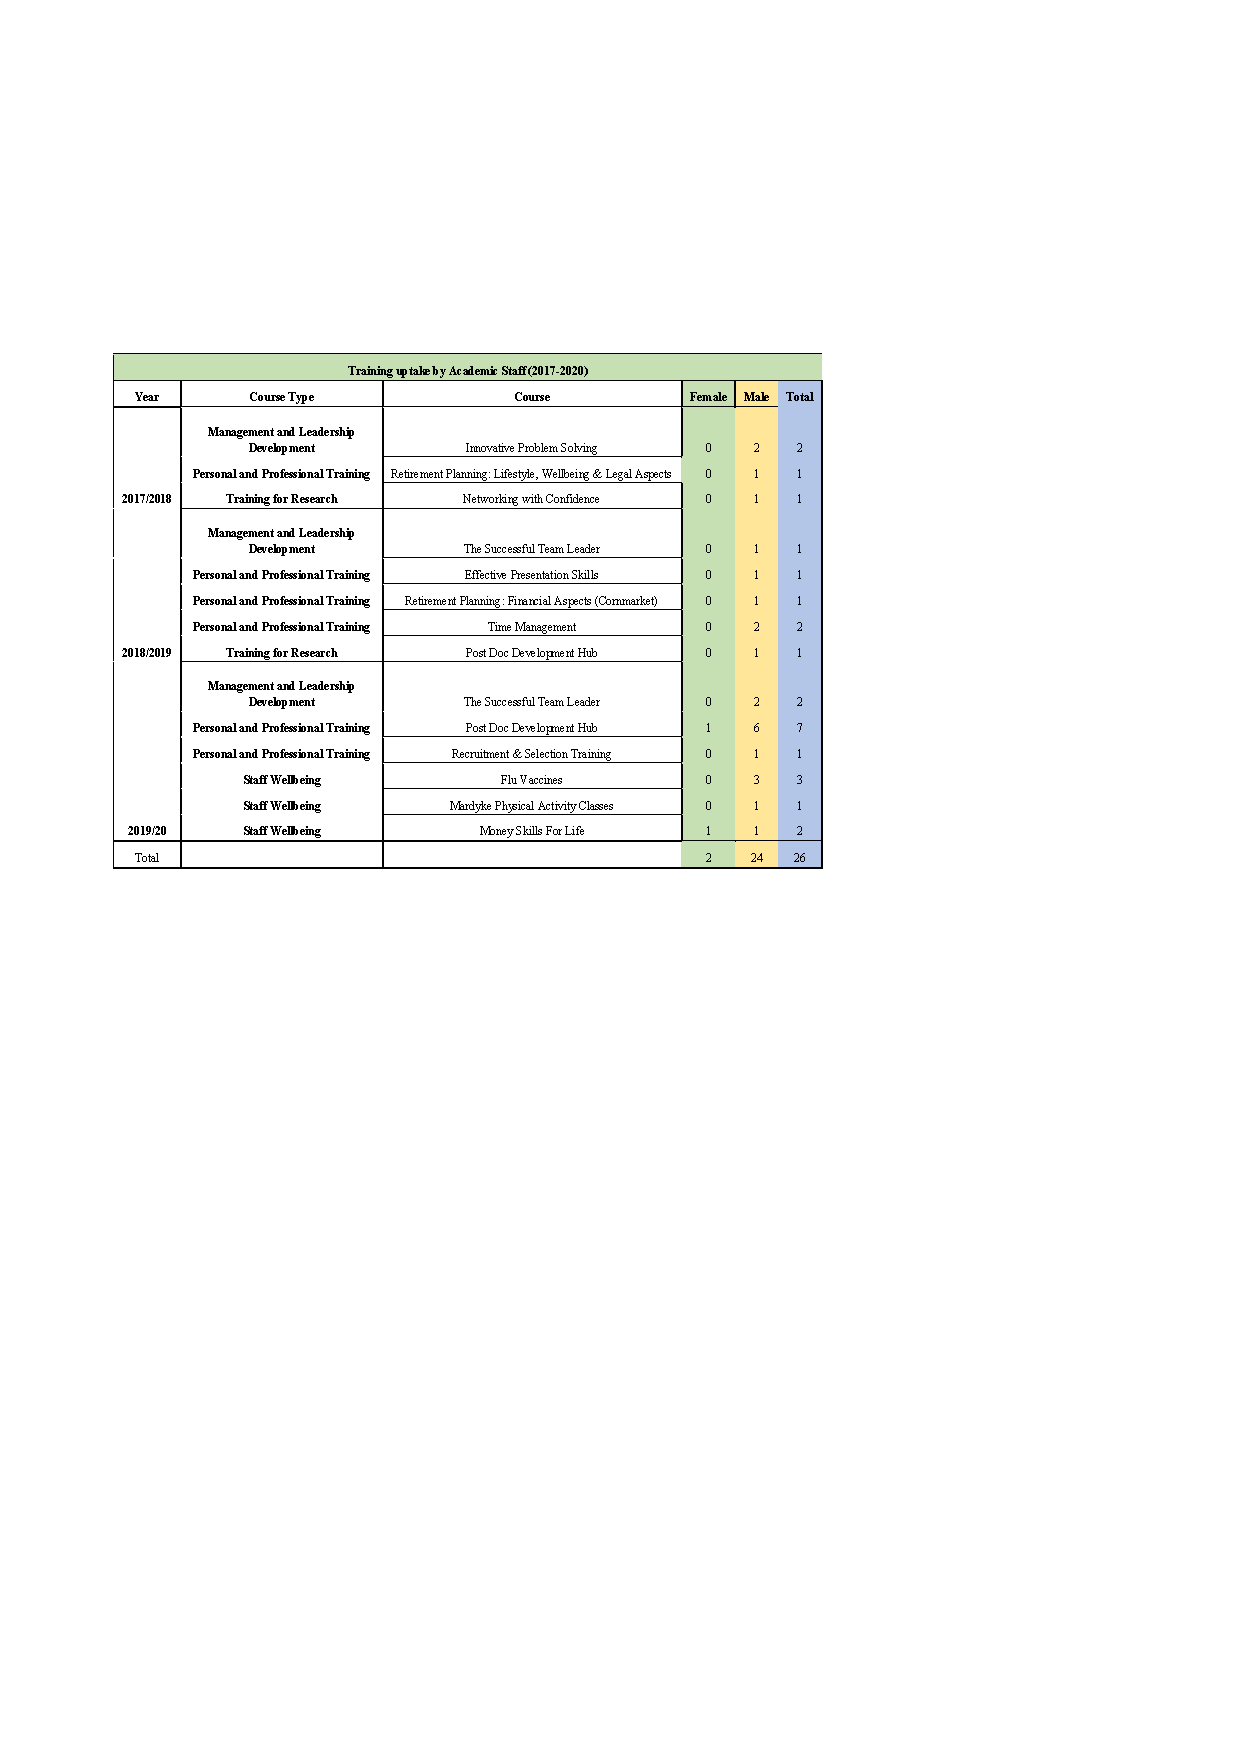
\includegraphics[width=\textwidth]{fig/table4.pdf}
%     \
% \end{table}

\begin{tabbox}{!th}
    \footnotesize 
    \caption{Training uptake by academic staff by gender}
    \label{tab:training:academic}
    %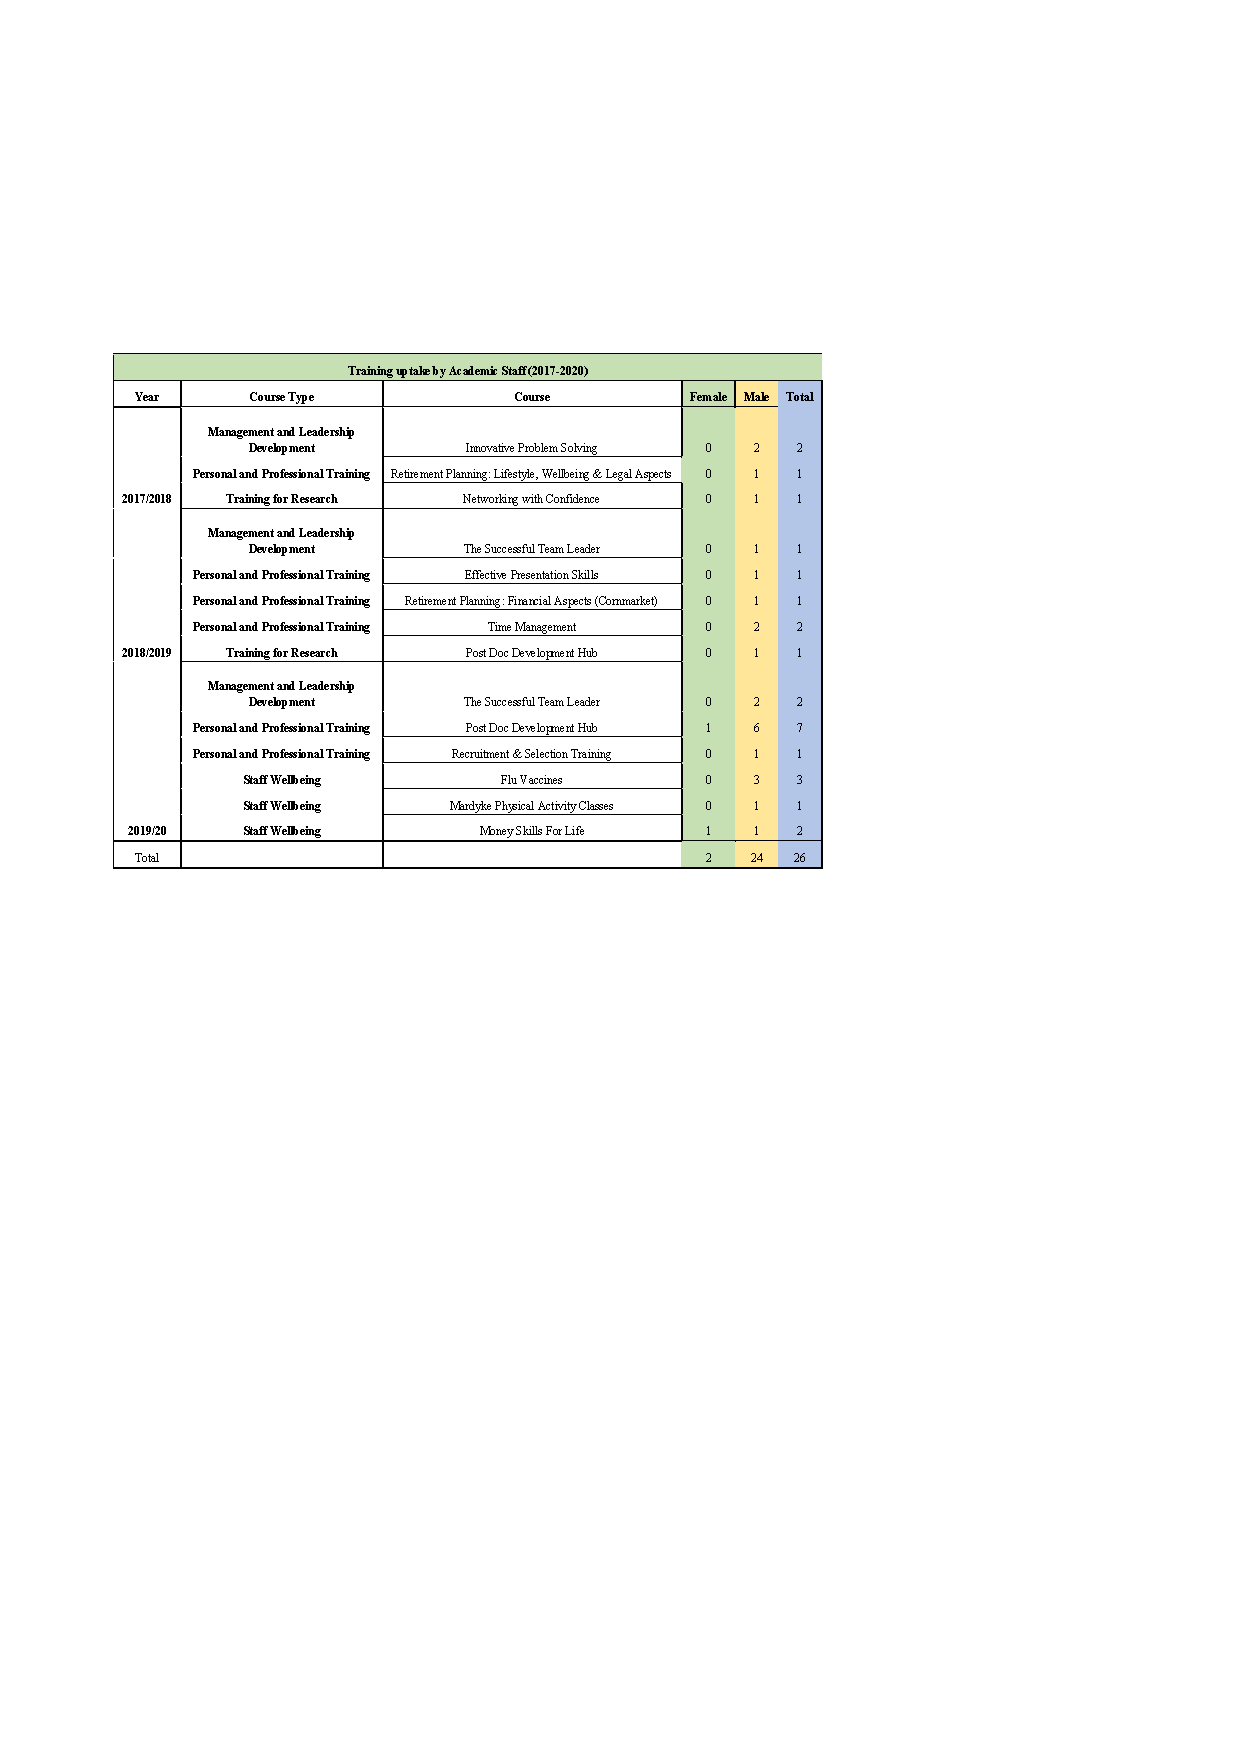
\includegraphics[width=\textwidth]{fig/table4.pdf}
    
    \begin{tabular}{p{2cm}
                    p{9.5cm}
                    !{\qquad}
                    R{1cm}
                    R{1cm}}
    
    \toprule 
    Year & Course & F & M \\
    \midrule
    
    2017/18 &  Innovative Problem Solving & 0 & 2\\
    \cdashline{2-4}
    & Retirement Planning: Lifestyle, wellbeing, and legal aspects & 0 & 1\\
    \cdashline{2-4}
    &  Networking with Confidence & 0 & 1\\
    \hdashline
    2018/19 &  The Successful Team Leader & 0 & 1\\
    \cdashline{2-4}
    & Effective Presentation Skills & 0 & 1 \\
    \cdashline{2-4}
    & Retirement Planning: Financial Aspects & 0 & 1 \\
    \cdashline{2-4}
    & Time Management & 0 & 2 \\
    \cdashline{2-4}
    & Post Doc Development Hub & 0 & 1 \\
    \hdashline
    2019/20 & The Successful Team Leader & 0 & 2 \\
    \cdashline{2-4}
    & Post Doc Development Hub  & 1 & 6 \\
    \cdashline{2-4}
    & Recruitment and Selection Training & 0 & 1 \\
    \cdashline{2-4}
    & Flu Vaccines & 0 & 3\\
    \cdashline{2-4}
    & Mardyke Physical Activity Classes  & 0 & 1\\
    \cdashline{2-4}
    & Money Skills for Life & 1 & 1\\
    \midrule 
    Total & & 2 & 24 \\
    
    \bottomrule      
         
    \end{tabular}
\end{tabbox}





Based on the staff survey, the majority of academic staff are aware of the PDRS process, with all female and 80\% of male staff being aware, whereas the majority of research staff are not aware of the PDRS process (Figure~\ref{fig:awareness}).
% Figure with awareness of PDRS process.

\begin{figbox}
    \caption{Awareness of the PDRS}
     %trim={<left> <lower> <right> <upper>}
    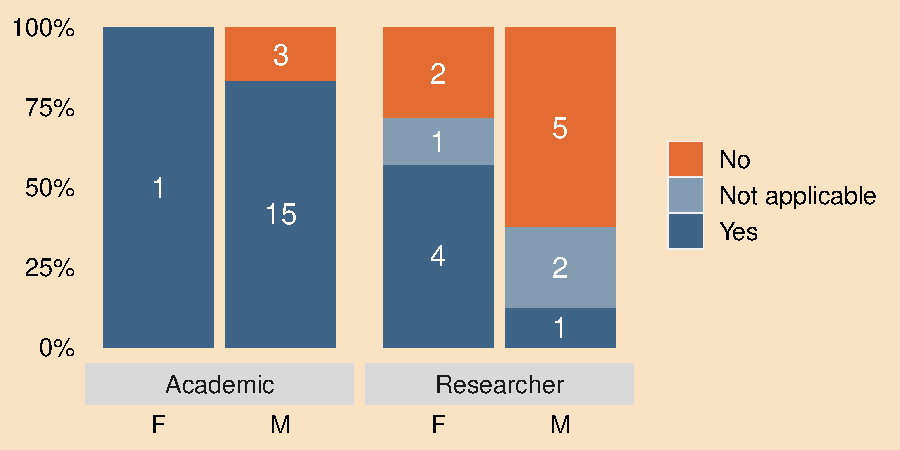
\includegraphics[trim={0 0 0 0},clip,width=14.2cm]{fig/awareness.pdf}
    \label{fig:awareness}
\end{figbox}




While the female academic staff member surveyed was very satisfied that she can discuss career progress and promotion opportunities with the
\ac{HOS}, approximately 15\% of male academic staff indicate that they are not satisfied (neutral to or disagree with) with those opportunities (see Figure~\ref{}). The planned action of restarting the PDRS process will hopefully address these concerns. % and give staff an opportunity to discuss their career development needs with the \ac{HOS}. 
Comments on the development process during the academic staff focus group were mixed:

\begin{myquote}
``The only conversations that I have with a line manager or head of department would be [about teaching schedules] ...''
\end{myquote}

\begin{myquote}
``The previous head of school ... he was very helpful. He tried to map out where are your weaknesses? [and supported me to develop in those areas]''
\end{myquote}

% Figure with career development opportinities - academic staff

\subsubsection{Training and Development Opportunities for Research Staff}
UCC, like all other Irish universities, considers postdoctoral staff as `research trainees' and provides through the PostDoc Development Hub (\url{https://www.ucc.ie/en/hr/research/devhub/}) a wide range of training and development offerings. Table~\ref{tab:training:postdoc} lists PostDoc Hub courses and their uptake by postdoctoral staff during the three years. While the data do not indicate how many researchers were availing of these, the uptake is rather limited, particularly among male researchers. 
%The data in Table~\ref{tab:training:researchstaff} overlaps with data from Table~\ref{tab:training:postdoc} to some extent. It shows overall a limited uptake of training and development opportunities by research staff in the school. 

\begin{figbox}
    \caption{Research staff career development}
     %trim={<left> <lower> <right> <upper>}
    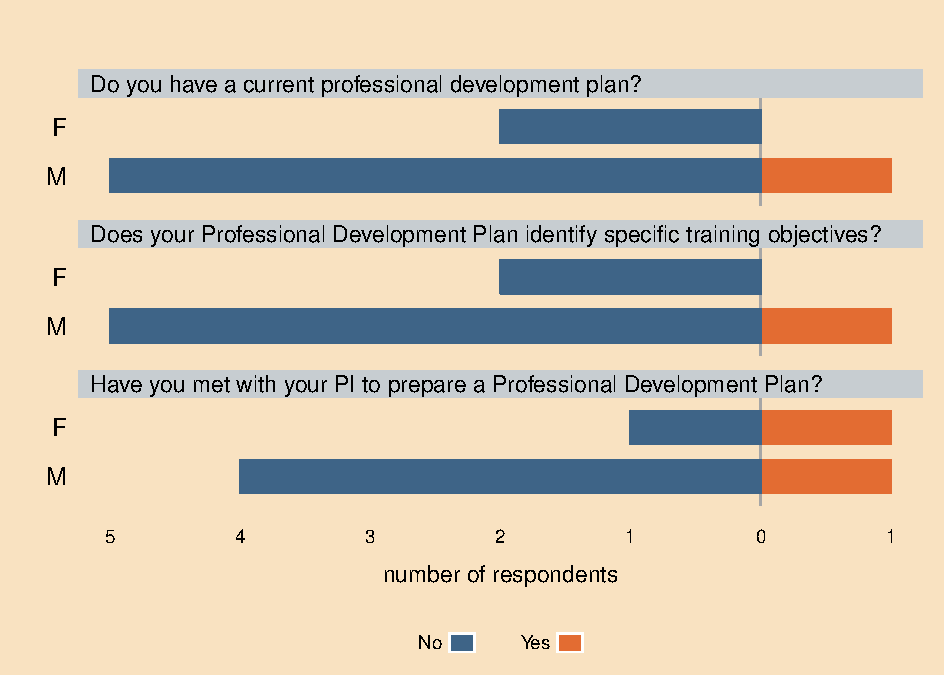
\includegraphics[trim={0 0 0 6mm},clip,width=9cm]{fig/researchcareerdev.pdf}
    \label{fig:research:career:development}
\end{figbox}



\begin{tabbox}{!th}
    
\caption{Training uptake by research staff by gender}
\label{tab:training:postdoc}
\footnotesize 

\begin{tabular}{p{1.5cm}
                p{9.5cm}
                R{1cm}
                R{1cm}}
    
    \toprule 
    Year & Course & F & M \\
    \midrule
    
    2017/18 & Developing and consolidating your career & 2 & 0\\
    \cdashline{2-4}
    & Project Management Part 1 & 1 & 0 \\
    \cdashline{2-4}
    & Project Management Part 2 & 1 & 0 \\
    \cdashline{2-4}
    & Grant Writing & 1 & 0 \\
    \cdashline{2-4}
    & Leading a Research Team & 1 & 0 \\
    \cdashline{2-4}
    & Research Data Management & 1 & 0 \\
    \hdashline
    2018/19  & Lean Yellow Belt Training & 1 & 1 \\
    \cdashline{2-4}
    & Active Listening Skills & 1 & 0 \\
    \cdashline{2-4}
    & Communicating With Impact - Managers/Team Leaders & 1 & 1 \\
    \cdashline{2-4}
    & Developing Positive and Assertive Communication Skills & 0 & 1 \\
    \cdashline{2-4}
    & Engaging People Who Are Anxious, Distressed, Angry & 0 & 2 \\
    \cdashline{2-4}
    & Identifying and Responding To Students In Distress & 0 & 1 \\
    \cdashline{2-4}
    & Managing Stress In The Workplace & 0 & 1 \\
    \cdashline{2-4}
    & The Effective Employee & 0 & 4 \\
    \cdashline{2-4}
    & Time Management & 0 & 2 \\
    \cdashline{2-4}
    & Unconscious Bias Training & 0 & 2 \\
    \cdashline{2-4}
    & Maximising Professional Effectiveness & 1 & 0 \\
    \cdashline{2-4}
    & Grant Writing & 0 & 1 \\
    \cdashline{2-4}
    & Presentation Skills & 1 & 10\\
    \cdashline{2-4}
    & Commercial Awareness and Knowledge Transfer & 0 & 1 \\
    \cdashline{2-4}
    & Data Management & 2 & 0 \\
    \cdashline{2-4}
    & Funding Your Research & 1 & 0 \\
    \cdashline{2-4}
    & Leading a Research Team & 1 & 0 \\
    \cdashline{2-4}
    & Managing Yourself Through Change & 1 & 0 \\
    \cdashline{2-4}
    & Statistics for Researchers & 1 & 0 \\
    \cdashline{2-4}
    & Teaching and Learning & 1 & 0 \\
    \hdashline
    2019/20 & Change Management & 0 & 1 \\
    \cdashline{2-4}
    & Communicating With Impact - Managers/Team Leaders & 1 & 0\\
    \cdashline{2-4}
    & Critical Thinking For Effective Decisions & 0 & 1 \\
    \cdashline{2-4}
    & Engaging People Who Are Anxious, Distressed, Angry & 1 & 0 \\
    \cdashline{2-4}
    & Flu Vaccines & 0 & 3 \\
\bottomrule      
\end{tabular}
    
\end{tabbox}


\begin{table}[!ht]
\colorbox{orangebg}{
    \begin{minipage}{14.2cm}
    \footnotesize 
    
    \begin{tabular}{p{1.3cm}
                    p{9.5cm}
                    R{1cm}
                    R{1cm}}
    
    \multicolumn{4}{l}{\textbf{Table~\thetable{}} Training uptake by research staff by gender (continued)}\\
    \toprule 
    Year & Course & F & M \\
    \midrule
    
       
    & Introduction To Project Management & 1 & 0 \\
    \cdashline{2-4}
    & Money Skills For Life & 1 & 1 \\
    \cdashline{2-4}
    & Networking Using Drama and Improvisation Techniques & 0 & 1 \\
    \cdashline{2-4}
    & Remote Working Workshop - Employee & 1 & 0\\
    \cdashline{2-4}
    & The Successful Team Leader & 0 & 2 \\
    \cdashline{2-4}
    & Time Management & 0 & 1 \\
    \cdashline{2-4}
    & UCC Health and Wellness Workshops & 1 & 0 \\
    \cdashline{2-4}
    & Winning The Stress Game - Stress Management Info Session & 1 & 1 \\
    \cdashline{2-4}
    & Project Management & 2 & 0 \\
    \cdashline{2-4}
    & Statistics for Researchers & 1 & 0 \\
    \cdashline{2-4}
    & Funding Your Research & 1 & 0 \\
    \cdashline{2-4}
    & Making That Transition & 1 & 0 \\
    \cdashline{2-4}
    & Presentation Skills for Research Staff & 1 & 1 \\
    \cdashline{2-4}
    & Motivation Skills for Research Staff & 1 & 0 \\
    \cdashline{2-4}
    & Communication Skills for Researchers & 1 & 0 \\
    \midrule 
    Total & & 34 & 29\\
    \bottomrule      
    \end{tabular}
    
\end{minipage} 
}

\end{table}

%%
\begin{table}[!ht]
\colorbox{orangebg}{
      \begin{minipage}{14.2cm}
\footnotesize 
    \caption{Training uptake by research staff}
    \label{tab:training:researchstaff}
    
    \begin{tabular}{p{1.3cm}
                    p{9.5cm}
                    R{1cm}
                    R{1cm}}
    
    \toprule 
    Year & Course & F & M \\
    \midrule
    


    
    \bottomrule      
         
    \end{tabular}
    
\end{minipage} 
}

\end{table}


% figure research career development


\begin{figbox}
    \caption{Academic career development opportunities}
    \includegraphics[width=14.3cm]{fig/acadcareer.pdf}
    \label{fig:acadcareerdev}
\end{figbox}

The feedback from the staff survey and research staff focus group was mixed in regard to career development (see Figure~\ref{fig:acadcareerdev}). The staff survey indicates that approximately 70\% of respondents indicated that they never had a meeting with their line manager (PI) to discuss their development needs. In fact, approximately 90\% said they did not currently have a personal development plan, 90\% indicated that they do not have training objectives and that of those, 67\% consider that they are not meeting their training objectives.
While this indicates a serious issue in regard to research staff development and training needs analysis, the participants commended the development opportunities available to them in UCC and felt supported within the School to avail of those opportunities (see Figure~\ref{fig:research:career:planning}). There is clearly much to do in supporting research staff with their development needs in general and female staff in particular to support them in developing a career in academia.  In order to address this, all PIs are strongly encouraged to promote and support their research staff in availing of the many training and career development opportunities available in UCC and to support them in the development of a Personal Development Plan (see Action~\ref{action:acad:cdp}).


   

               
\begin{figbox}
    \caption{Support for researcher career planning}
    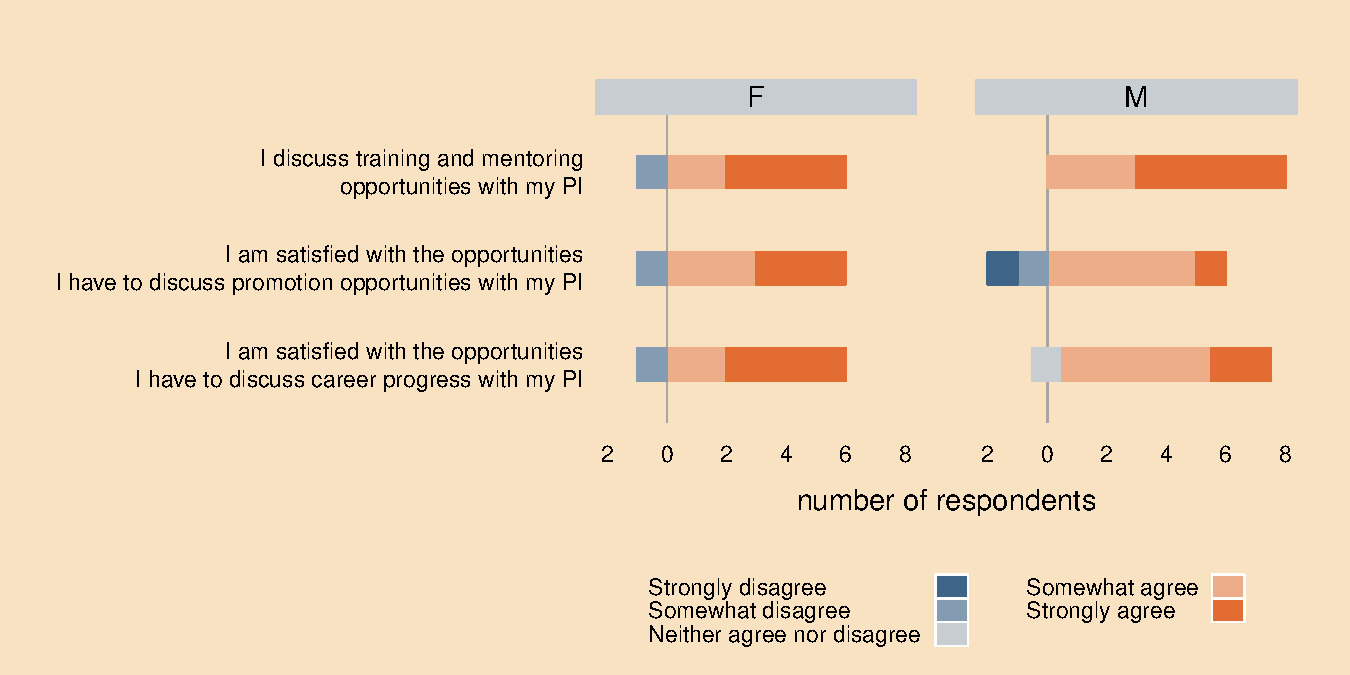
\includegraphics[trim={8mm 3mm 10mm 1cm },clip,width=14.2cm]{fig/figrescardev.pdf}
    \label{fig:research:career:planning}
\end{figbox}



% figure support research career planning



\newcommand{\actacadcdp}{%Action 2.8 
Organise series of bespoke workshops for specific staff career planning.}
\begin{actionblock}{\ksspace{}Bespoke Workshops for Staff Career Planning}{acad:cdp}
\actacadcdp
\hfill{
    \hypersetup{hidelinks}
    \hyperlink{c14}{\gotoactionsymbol{}}
}
\end{actionblock}


% Section 2.2.f

\subsection{Comment and reflect on department engagement with institution-level supports for academic and research staff career progression as well as any department-level support available. This should include results from staff consultation presented by gender and may include, but is not limited to, support given to staff to:}\label{sec:2f}
\instr{
\begin{itemize}
\item	apply for research funding;
\item	develop excellence in teaching and learning.
\end{itemize}
}

%\subsubsection{Department's engagement with institution-level supports for staff career progression}
\subsubsection{Support for Training and Development}
%As pointed out in the previous section, many staff are not fully aware of the development opportunities available to support career progression in UCC. 
%While there are negative views on the promotion process, supports to help a staff member to develop their career exist. 
The School has no formal support for career progression.  
Most male respondents to the staff survey mentioned they were not aware of the relevance or availability of training opportunities, whereas female respondents did. Many male respondents indicated to be dissatisfied with the support from the \ac{HOS} to participate in training opportunities, whereas female staff indicated to be satisfied. 
Further, some male academic staff shared negative comments on the support they received from the school to attend conferences or present their work to others in the School
%The staff survey indicated that the majority of the surveyed male academic staff mentioned that they are not aware of the relevance or availability of training opportunities, whereas the female staff states awareness. 
%Many of the surveyed male academic staff indicated that they are not satisfied with the support they receive from the HoS for participation in training opportunities, whereas the surveyed female staff are satisfied.
%There were also negative comments by male academic staff on the support they receive from the School to attend conferences or present their work to others in the School 
(see Figure~\ref{fig:training}).


\begin{figbox}
    \caption{Training awareness}
    % left lower right upper
    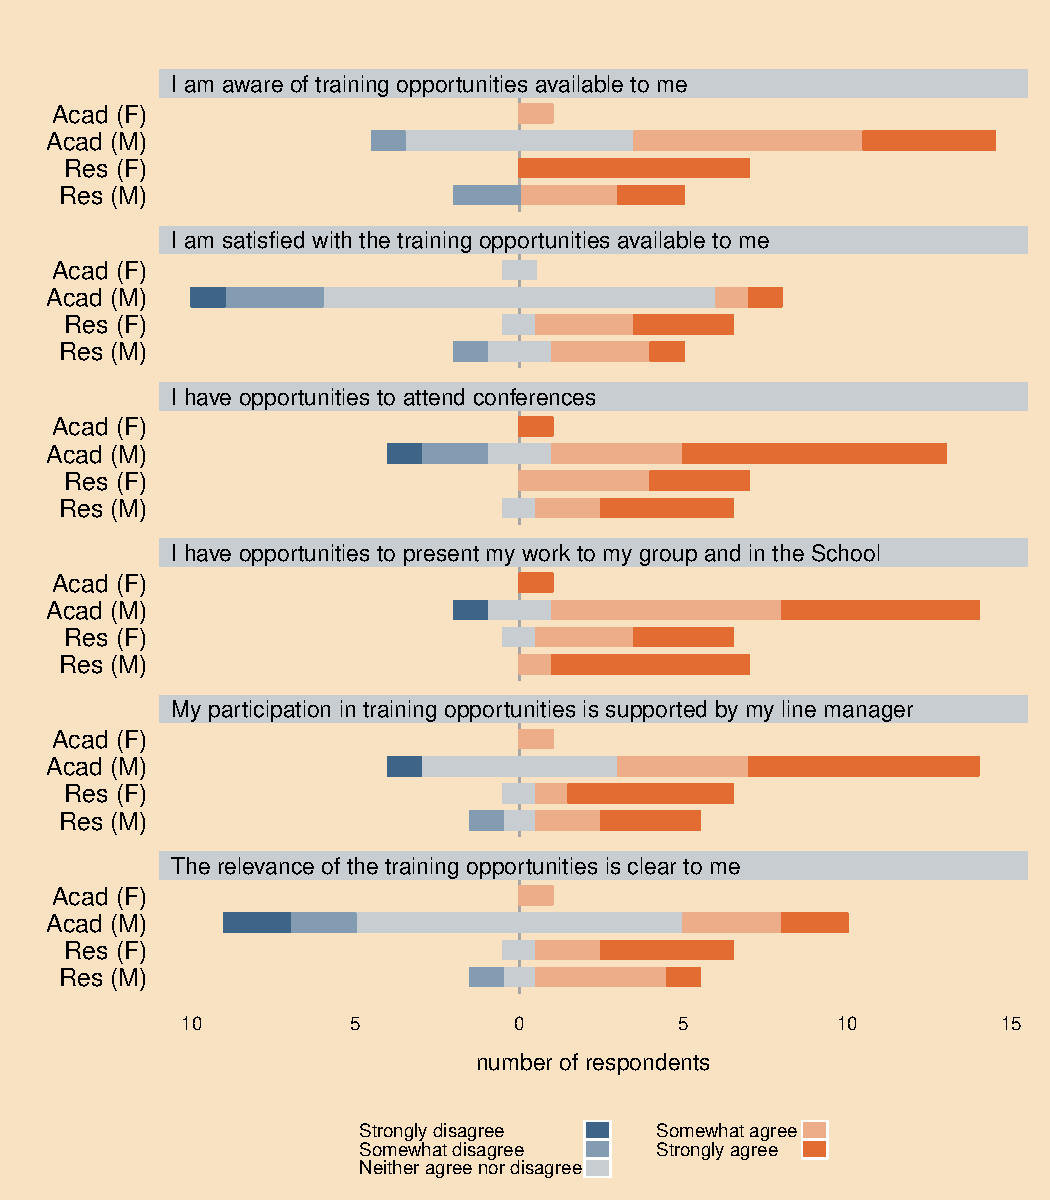
\includegraphics[trim={0mm 2mm 0 10mm},clip,width=14.2cm]{fig/training.pdf}
    \label{fig:training}
\end{figbox}



%Figure Staff Training Awareness


%The staff survey showed a somewhat different picture for research staff. 
For research staff, a number of issues were identified:
\begin{itemize}[itemsep=0pt]
\item Lack of awareness of training opportunities;
\item Lack of relevance of training opportunities;
\item Lack of satisfaction with available training opportunities;
\item Perceived lack of support by line manager to participate in training opportunities;
\item Perceived lack of opportunity to attend conferences (males only)
\item Perceived lack of opportunity to present their work to peers or in the School (females only).
\end{itemize}

%Some male research staff indicated that they were not aware of the training opportunities available to them. Others, both female and male, did not see the relevance of available training opportunities, and a similar number of research staff indicated not being satisfied with the available training opportunities. Some research staff, both male and female, felt that they were not supported by their line manager to participate in training opportunities. Some male research staff did not feel they had sufficient opportunity to attend conferences, whereas all surveyed female research staff were satisfied with their opportunities. On the other hand, some female research staff felt they did not have enough opportunity to present their work to peers or in the School, whereas all male research staff were satisfied with their opportunities. 
Comments from the staff survey indicated a need for better communication on training and staff development opportunities within the School:

\begin{myquote}
``It's important to keep training to keep up to date. I'd like more open discussion around training needs and requirements.''
\end{myquote}

\begin{myquote}
“Unfortunately, I have never heard or seen any email where funding for training has been circulated or promoted.''
\end{myquote}

Comments received from the academic staff focus group indicated satisfaction  %\todo{those who attended} 
with the support received from the School. They were satisfied with the training offered centrally, but commented on their perception that the uptake among academic staff seems low. Others suggested better information on and promotion of training opportunities through the School:

\begin{myquote}
``Those kind of courses [like CIRTL – Centre for Integration of Research, Teaching, and Learning] should be advertised by the department … courses that we can improve … project management skills, soft skills, hard skills … I think that would really benefit us going forward.''
\end{myquote}

Participants in the research staff focus group indicated a need for more support for research staff development at School level. 
Most of the support for career development was coming through their respective research centres and groups rather than the School. 
This results in varying experiences among researchers; some researchers said that those not in centres or groups often ended up isolated. The School clearly needs to raise the awareness of training opportunities available to all staff to help them with career development (see Action~\ref{action:acad:cdpawareness} and Action~\ref{action:acad:localsupport}).

\newcommand{\actcdpawareness}{%Action 2.18 
Increase awareness of existing menue of career development support.}
\begin{actionblock}{\ksspace{}Awareness of Career Development Support}{acad:cdpawareness}
\actacadpdrs
\hfill{
    \hypersetup{hidelinks}
    \hyperlink{c13}{\gotoactionsymbol{}}
}
\end{actionblock}

\newcommand{\actacadlocalsupport}{%Action 2.21 
Improve communication and enhance local support for career development opportunities available to staff.}
\begin{actionblock}{\ksspace{}Enhance Local Support for Career Development}{acad:localsupport}
\actacadlocalsupport
\hfill{
    \hypersetup{hidelinks}
    \hyperlink{c18}{\gotoactionsymbol{}}
}
\end{actionblock}

\subsubsection{Support in Research Funding Applications}
The staff survey indicated a need for more support from the School for research funding applications (see Figure~\ref{fig:fundingsupport}). A number of issues were revealed among academic staff:

\begin{itemize}
    \item Female respondents expressed dissatisfaction with opportunities to apply for research funding, as did half of the male respondents;
    \item Female academics were satisfied with support for research funding applications provided by the \ac{OVPRI} and the College's Research Support Office, but half of male respondents were not;
    \item Most respondents indicated a dissatisfaction with the support provided by the School to staff whose research funding applications were unsuccessful. 
\end{itemize}



Among research staff, we identified the following issues:

\begin{itemize}
    \item A third of female and the majority of male research staff were not satisfied with the opportunities they had to apply for research funding. This may be partly due to eligibility criteria by some funding agencies, who require a certain length of contract for some of their schemes;
    \item A third of female and half of male respondents were dissatisfied with the support offered by the School in applying for research funding; fewer female respondents indicated the same dissatisfaction with support from \ac{OVPRI}. 
    \item Similar numbers indicated dissatisfaction with support from the School to staff whose research funding applications were rejected.
\end{itemize}


\begin{figbox}
    \caption{Support for funding}
    % left lower right upper
    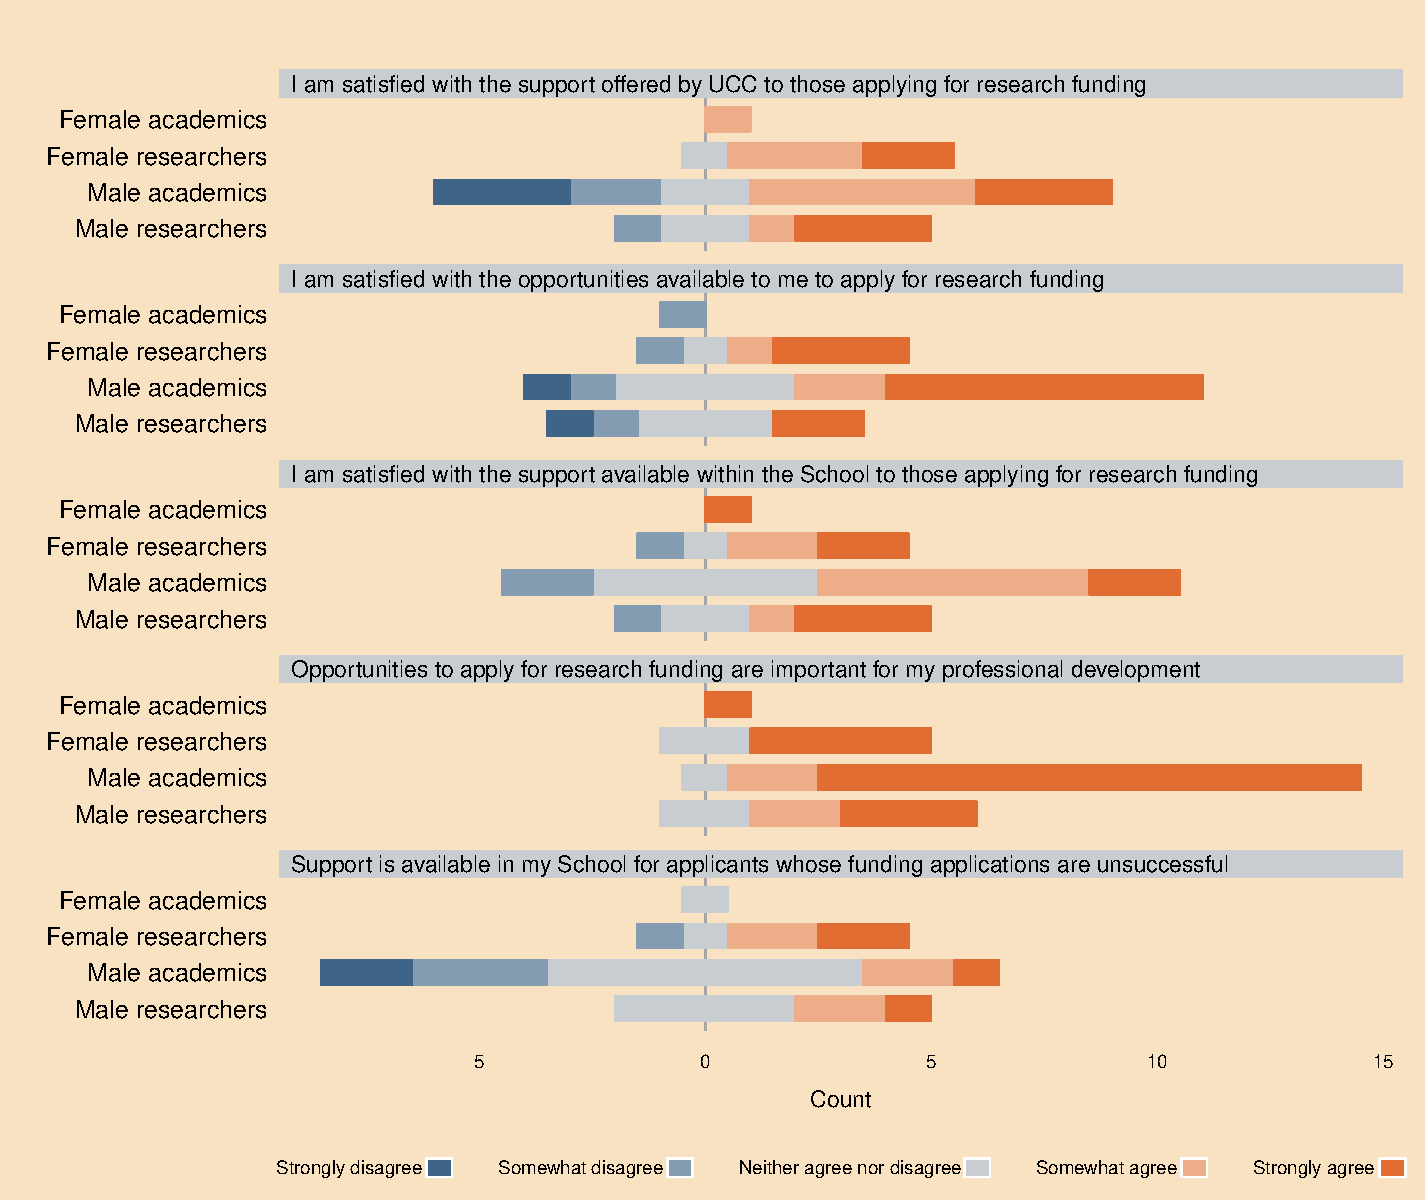
\includegraphics[trim={6mm 0 0 0},clip,width=14.5cm]{fig/fundingsupport.pdf}
    \label{fig:fundingsupport}
\end{figbox}



%All surveyed female academic staff were dissatisfied with the opportunities they have to apply for research funding, whereas almost half of male respondents indicated the same. 
%Perceptions of support for research funding applications also varied; all female academic staff indicated satisfaction, but half of the male respondents indicated dissatisfaction.
%Central support for research funding applications is provided by the \ac{OVPRI} and the College's Research Support Office. 
%All female academic staff were satisfied with these supports, whereas a little under half of male academics were not. 
%All female and almost all male academic staff indicated they were not satisfied with the support the School provides to staff whose research funding applications were unsuccessful. 
Success in attracting research funding is a key factor in academic career progression and the School clearly needs to provide sufficient support to academic staff in identifying opportunities and developing funding proposals (see Action~\ref{action:acad:supportfunding}). 

\newcommand{\actacadsupportfunding}{%Action 2.11 - support junior female staff - similar to promotion
Create a support programme at School level to support staff with research funding applications.}
\begin{actionblock}{\ksspace{}Research Funding Support Programme}{acad:supportfunding}
\actacadsupportfunding
\hfill{
    \hypersetup{hidelinks}
    \hyperlink{c16}{\gotoactionsymbol{}}
}
\end{actionblock}

%and help in particular female academic staff with identifying opportunities for research funding applications and then help with the application process to increase success rate.
%
% Figure ResearchFundingSupport
%
%About a third of female and the majority of male research staff were not satisfied with the opportunities they had to apply for research funding. This may be partly due to eligibility criteria by some funding agencies, who require a certain length of contract for some of their schemes. 
%A third of female and nearly half of male research staff were not satisfied with the support the School provides them with when applying for research funding, although fewer female research staff  indicated the same dissatisfaction with support from \ac{OVPRI}, the number of male staff dissatisfied remained the same. 
%A third of female and the majority of male research staff indicated they were not satisfied with the support the School provides to staff whose research funding applications were unsuccessful. 
%Clearly, more effort is needed by the school to support the both academic and research staff in applying for funding applications (see Action~\ref{action:acad:supportfunding}).

\subsubsection{Support in Teaching}
Academic survey respondents  were broadly satisfied with access to and support for equipment and digital tools to support teaching, including laboratories. In particular, the IT support group in the school is held in high esteem. % and provides excellent support within budget constraints. 
During the research staff focus group, participants commented that improving communication with researchers about opportunities to participate in tutoring, demonstrating, and lecturing, would be helpful. 
A lack of awareness and information might be stopping interested researchers from availing of existing teaching opportunities.






\subsection{Comment and reflect on how workload is allocated and managed in the department (e.g. via a workload allocation model). This should include information on how the breadth of academic and research roles and responsibilities are captured in workload planning and allocation and results from staff consultation presented by gender.}\label{sub:workload}

Academic workload includes teaching, research, and administrative work 
While research staff are primarily conducting research, depending on their role and seniority their workload may include some administrative work.
%whereas research staff workload is largely concentrated on research work but depending on role and seniority may include some administrative work. 
Research workload for academic staff varies by staff member, depending on their interests and motivation. There is no assigned research workload by the \ac{HOS}. 
%The workload that is assigned and agreed between an academic staff member and the HoS includes teaching assignment and some administrative tasks. 
%The current practice in the school in regard to teaching workload is that 
Most academic staff carry the same workload of 20 ECTS per academic year, which usually translates to four modules. 
Academic staff are asked for their preference to teach specific modules, and the allocation seeks to satisfy these preferences as best as possible. In addition, all staff are asked to supervise up to 6 student projects across all taught programmes. Some staff may be assigned a lower teaching load of 15 credits, but in return are assigned  a higher number of students to supervise. 
%This practice has an exception for very research active staff who supervise/co-supervise more than 10 PhD students. Those staff’s teaching allocation is reduced by five credits (one module). Currently, there are only three academic staff members, all male, who have a reduced teaching load. Additionally, new 
New staff are assigned a reduced teaching load of 15 credits for their first year in the school to enable them to settle in and start developing their research agenda.

Administrative tasks include membership and chairing roles in a number of school  committees (see Section~\ref{sec:overview}). %, many of which are replicated at College level and require the chair to attend the College level committee as well. 
The allocation process seeks expressions of interest and preferences from academic staff for the position of chair or member of committees, and the HoS  attempts to meet those preferences as best as possible. 
%As chairs often have a higher workload than committee members, the workload can be uneven depending on the role. 

Academic course directorships carry more administrative load and these tend to rotate every few years.  There is currently very limited recognition of research workload in regard to academic and administrative workload allocation, which creates a higher workload for research active staff compared to those who conduct less research. There is currently also no recognition of caring responsibilities in allocation of workload.

Workload allocation for research staff depends on their line manager and depends to some extent on the respective staff member's ambitions. The current contract for research staff specifies a 37-hour work-week. There is no information available on how many hours per week academic and research staff actually work. Consultation of academic staff in regard to workload allocation through the staff survey and focus group yielded a diverse response. 

\subsubsection{Academic workload model}
% Insert Figure on Workload Allocation Model
Just under half of the male academic staff indicated familiarity with UCC's workload allocation model, whereas the single female staff member respondent indicated no familiarity (see Figure~\ref{fig:workloadallocmodel}). Over half the male staff indicated they do not understand its purpose, while the female staff indicated that she understands its purpose. However, almost all staff, female and male, were unaware of its outcomes nor did they consider it transparent or fair. Clearly, an action is required to create a clear, fair and transparent workload model in the School to support all staff (see Action~\ref{action:acad:transparentworkload}).

\begin{figbox}
   \caption{Workload Distribution Model (WDM)}
    % left lower right upper
    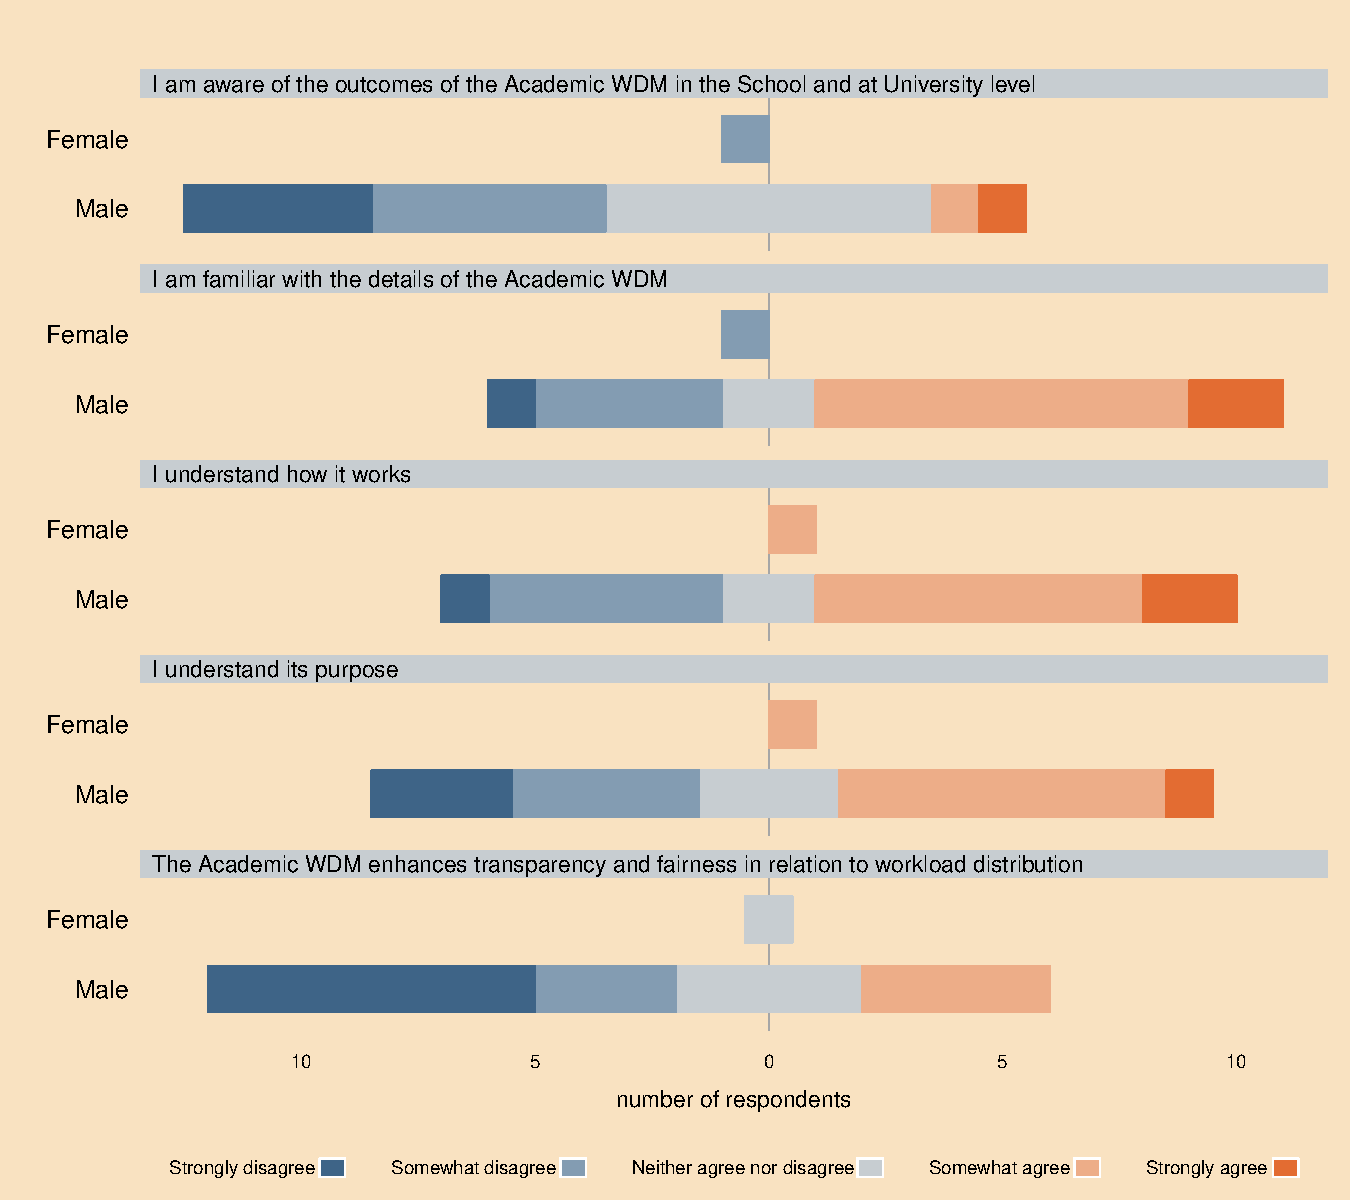
\includegraphics[trim={6mm 0 0 0},clip,width=14.2cm]{fig/workloadallocationmodel.pdf}
    \label{fig:workloadallocmodel}
\end{figbox}


\begin{figbox}
    \caption{Workload}
    % left lower right upper
    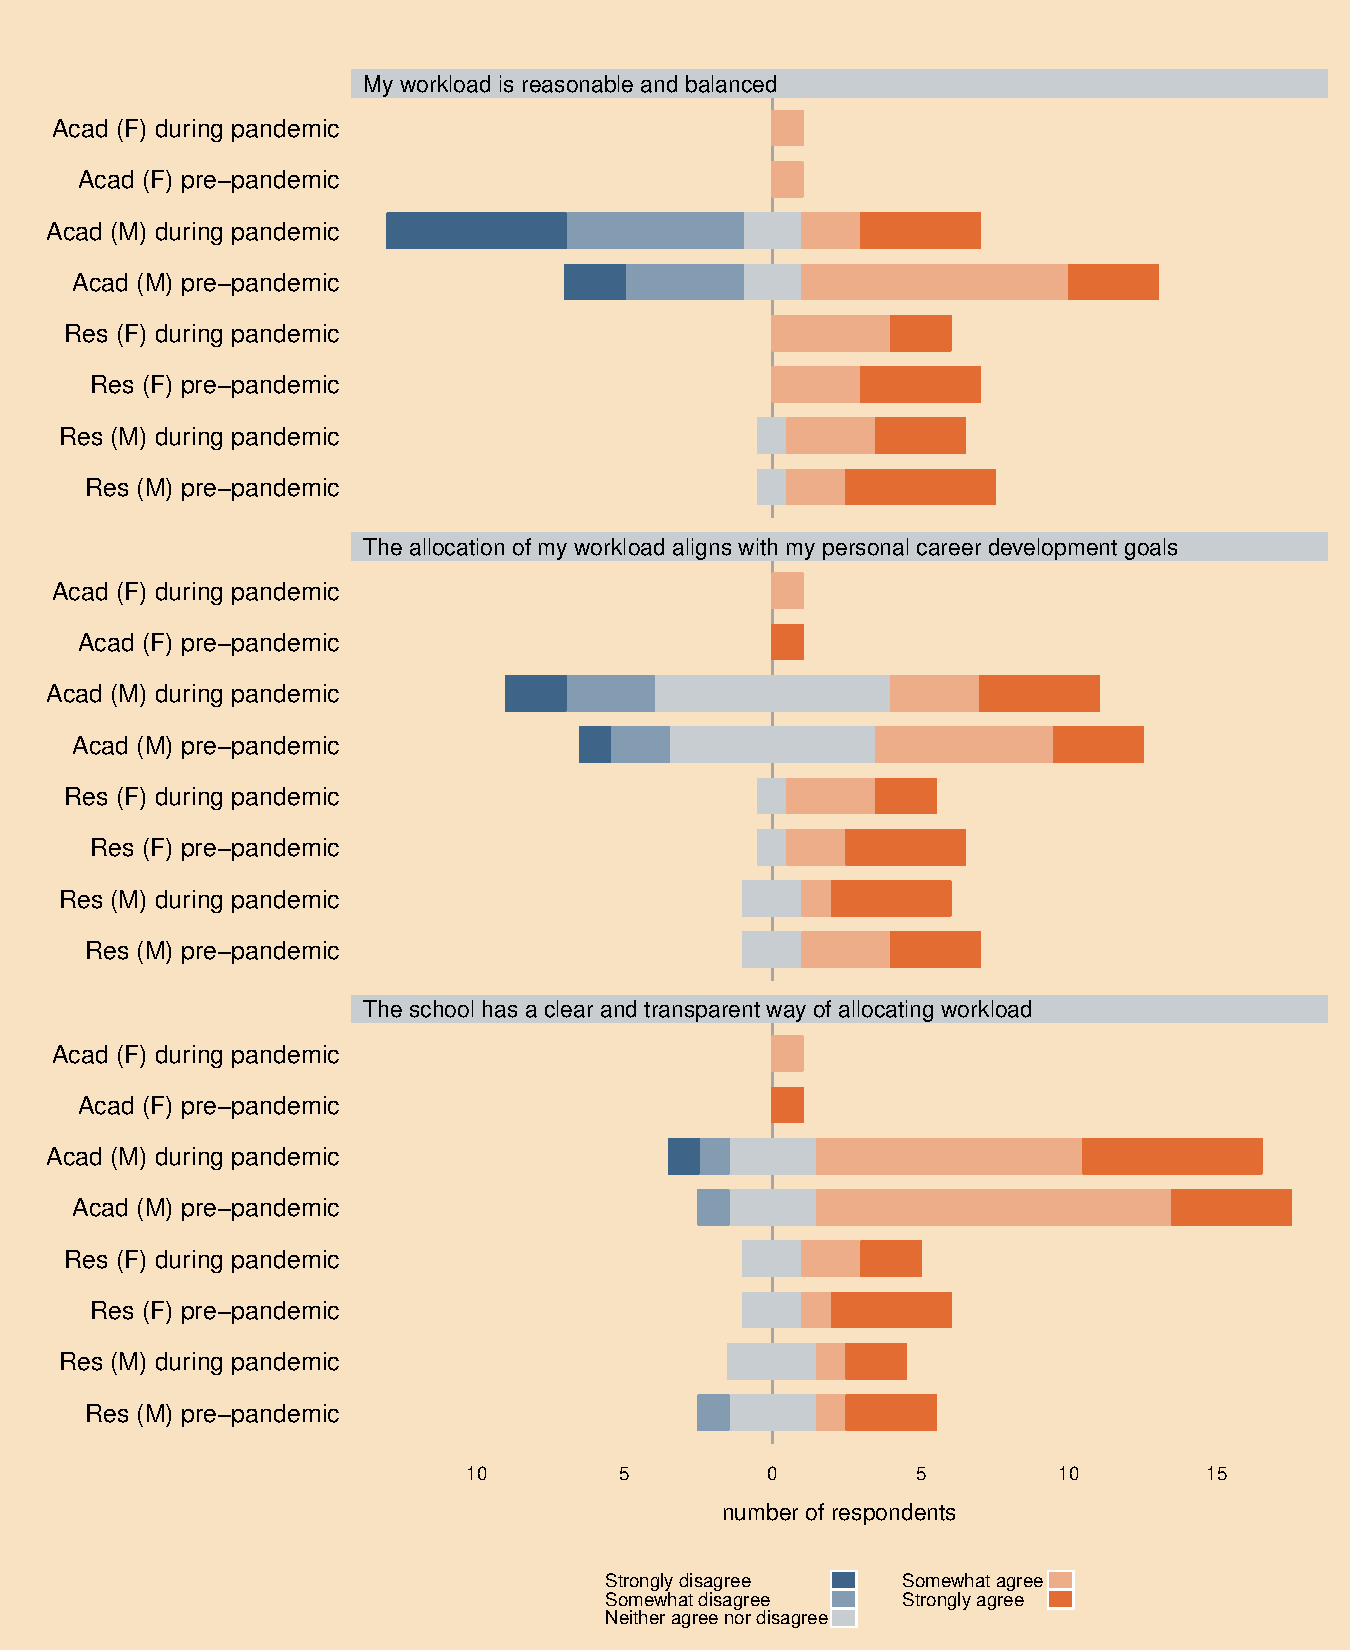
\includegraphics[trim={0 0 0 0},clip,width=14cm]{fig/workload.pdf}
    \label{fig:workload}
\end{figbox}

\begin{figbox}
    \caption{Perceived changes to workload}
    % left lower right upper
    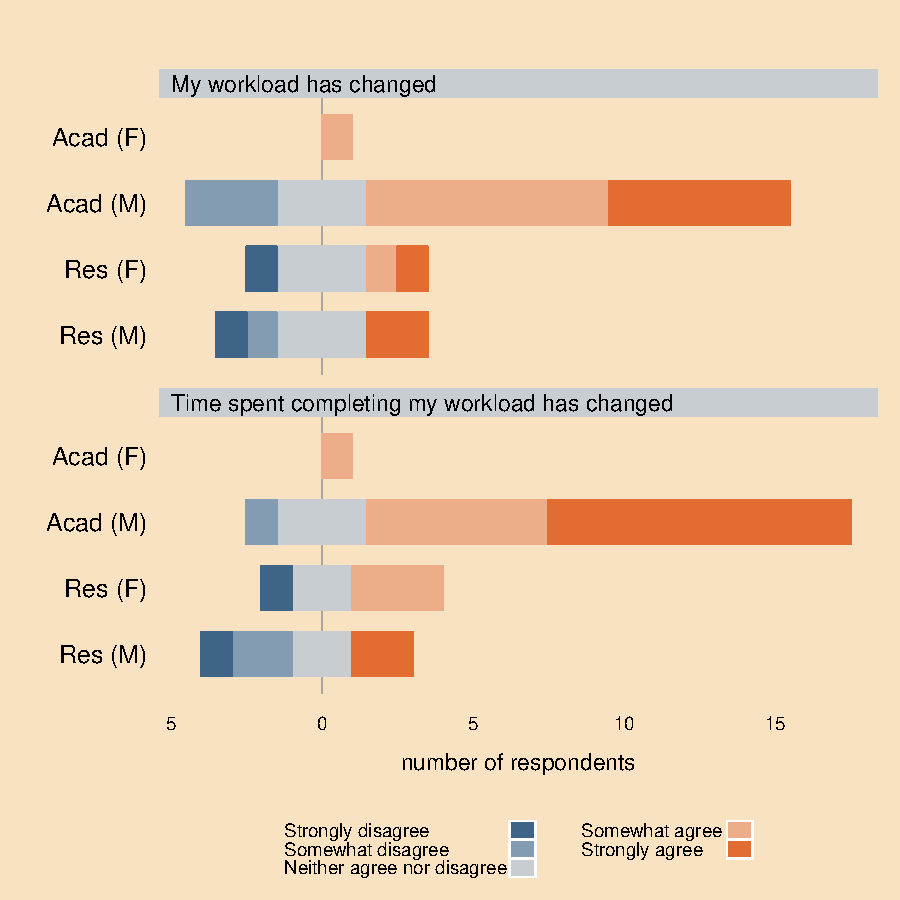
\includegraphics[trim={6mm 0 0 10mm},clip,width=10cm]{fig/workload2.pdf}
    \label{fig:workloadchange}
\end{figbox}




\subsubsection{Workload allocation and management}
% Insert Figure on Workload
The female respondent felt that her workload was reasonable and balanced and that the School has a clear way of allocating it and that it aligns with her career goals. This has not changed during the Covid-19 period (Figure~\ref{fig:workload}). %, however, due to the limited response of female academic staff, it is unclear if this view is representative. 
Among male academic staff, just over half felt their workload allocation was reasonable and balanced; the majority felt that the allocation was clear and transparent. Only half said that the workload allocation aligned with their personal career development goals. Most male respondents felt that their workload was not balanced and had changed since the pandemic started. During the academic focus group session, some colleagues commented on ever-increasing administrative tasks and scheduling of meetings and academic tasks that negatively affect caring responsibilities. %, such as the collection of children from childcare between 5-6pm.

% \begin{myquote}
% “It’d a full-time job, just to attend all the meetings, from college meetings, to department meetings, … -- it’s just overkill. ...”
% \end{myquote}

\begin{myquote}
“Caring responsibilities are not considered when it comes to timing of meetings or academic responsibilities e.g. lecturing/labs. It is also not considered for workload. Furthermore, if it were to be considered, I strongly suspect it would impact career progression as, simply put, those without caring responsibilities would have higher quantitative output e.g. published papers, international collaborations etc.”
\end{myquote}

Among research staff, both female and male respondents felt that their workload was reasonable and balanced (see Figure~\ref{fig:workload}), whereas 50\% of both female and male staff did not consider that the way workload is allocated is clear and transparent. Again the majority of staff, female and male, felt that the allocated workload aligned with the career development goals. Specific comments from surveyed staff mentioned that \textit{“If anything, the workload has increased considerably in the past 16 months”} but that \textit{“teamwork is good.”}


\subsubsection{Work-Life Balance}
% Insert Figure on Work-Life Balance

Academic survey respondents were generally negative about work-life balance. Again, the response from the single female academic staff member was that her work-life balance was satisfactory, that she felt comfortable discussing it with the HoS and thought the HoS would address any issues. In contrast, the vast majority of male respondents were dissatisfied with their work-life balance, although the majority were comfortable discussing it with the HoS and thought that the HoS would act on concerns. Comments from the survey indicated that the workload can also be self-imposed and that this is not specific to the School of CSIT:

\begin{myquote}
``It is hard for academic staff to clearly define work-life balance, as our work can be driven by our ambitions as much as by what is asked of us. A significant part of our work is self-motivated and defined by ourselves, without line management influence.''
\end{myquote}

% \begin{myquote}
% “The academic culture does not support work-life balance, and this badly needs to be addressed. I would like to emphasise that this is not specific to the School of Computer Science but is a culture across the university and within academia. 
% Every effort should be made to reduce administrative or unnecessary workload on those with additional caring responsibilities and ensure fair distribution across all individuals.”
% \end{myquote}

Researchers who responded to the survey, both male and female, indicated that they are by and large happy with their work-life balance. All felt that they could discuss issues with their line manager, but expressed less certainty whether actions would be taken. Research focus group participants described a supportive culture in research centres to meet staff needs for flexible working, which helps those with caring obligations. 


\newcommand{\actacadtransparentworkload}{%Action 2.12 - to help all to reach full potential-  ties back to personal development
Review workload model for academic and research staff.}
\begin{actionblock}{\ksspace{}Review Workload Model}{acad:transparentworkload}
\actacadtransparentworkload
\hfill{
    \hypersetup{hidelinks}
    \hyperlink{c19}{\gotoactionsymbol{}}
}
\end{actionblock}

%\newcommand{\actacadnewworkload}{%Action 2.22 
%Improve workload allocation based on new workload model.}
%\begin{action}[label=action:acad:newworkload]{}
%\actacadnewworkload
%\hfill{
%    \hypersetup{hidelinks}
%    \hyperlink{c20}{\gotoactionsymbol{}}
%}
%\end{action}


%% End of section.
